\section{The primary sequence of \protein{Mad1}'s loop region is not conserved but the secondary structure is}
% To understand which model is correct/design an experiment to prove which hypothesis is correct in a more direct way (or at least from a different angle), we need to understand the structure of MAD1 first.
% The algorithm originally proposed in \cite{LupasCOILS} predict regions of discontinuity within coiled-coil structures.

\begin{figure}
    \centering
    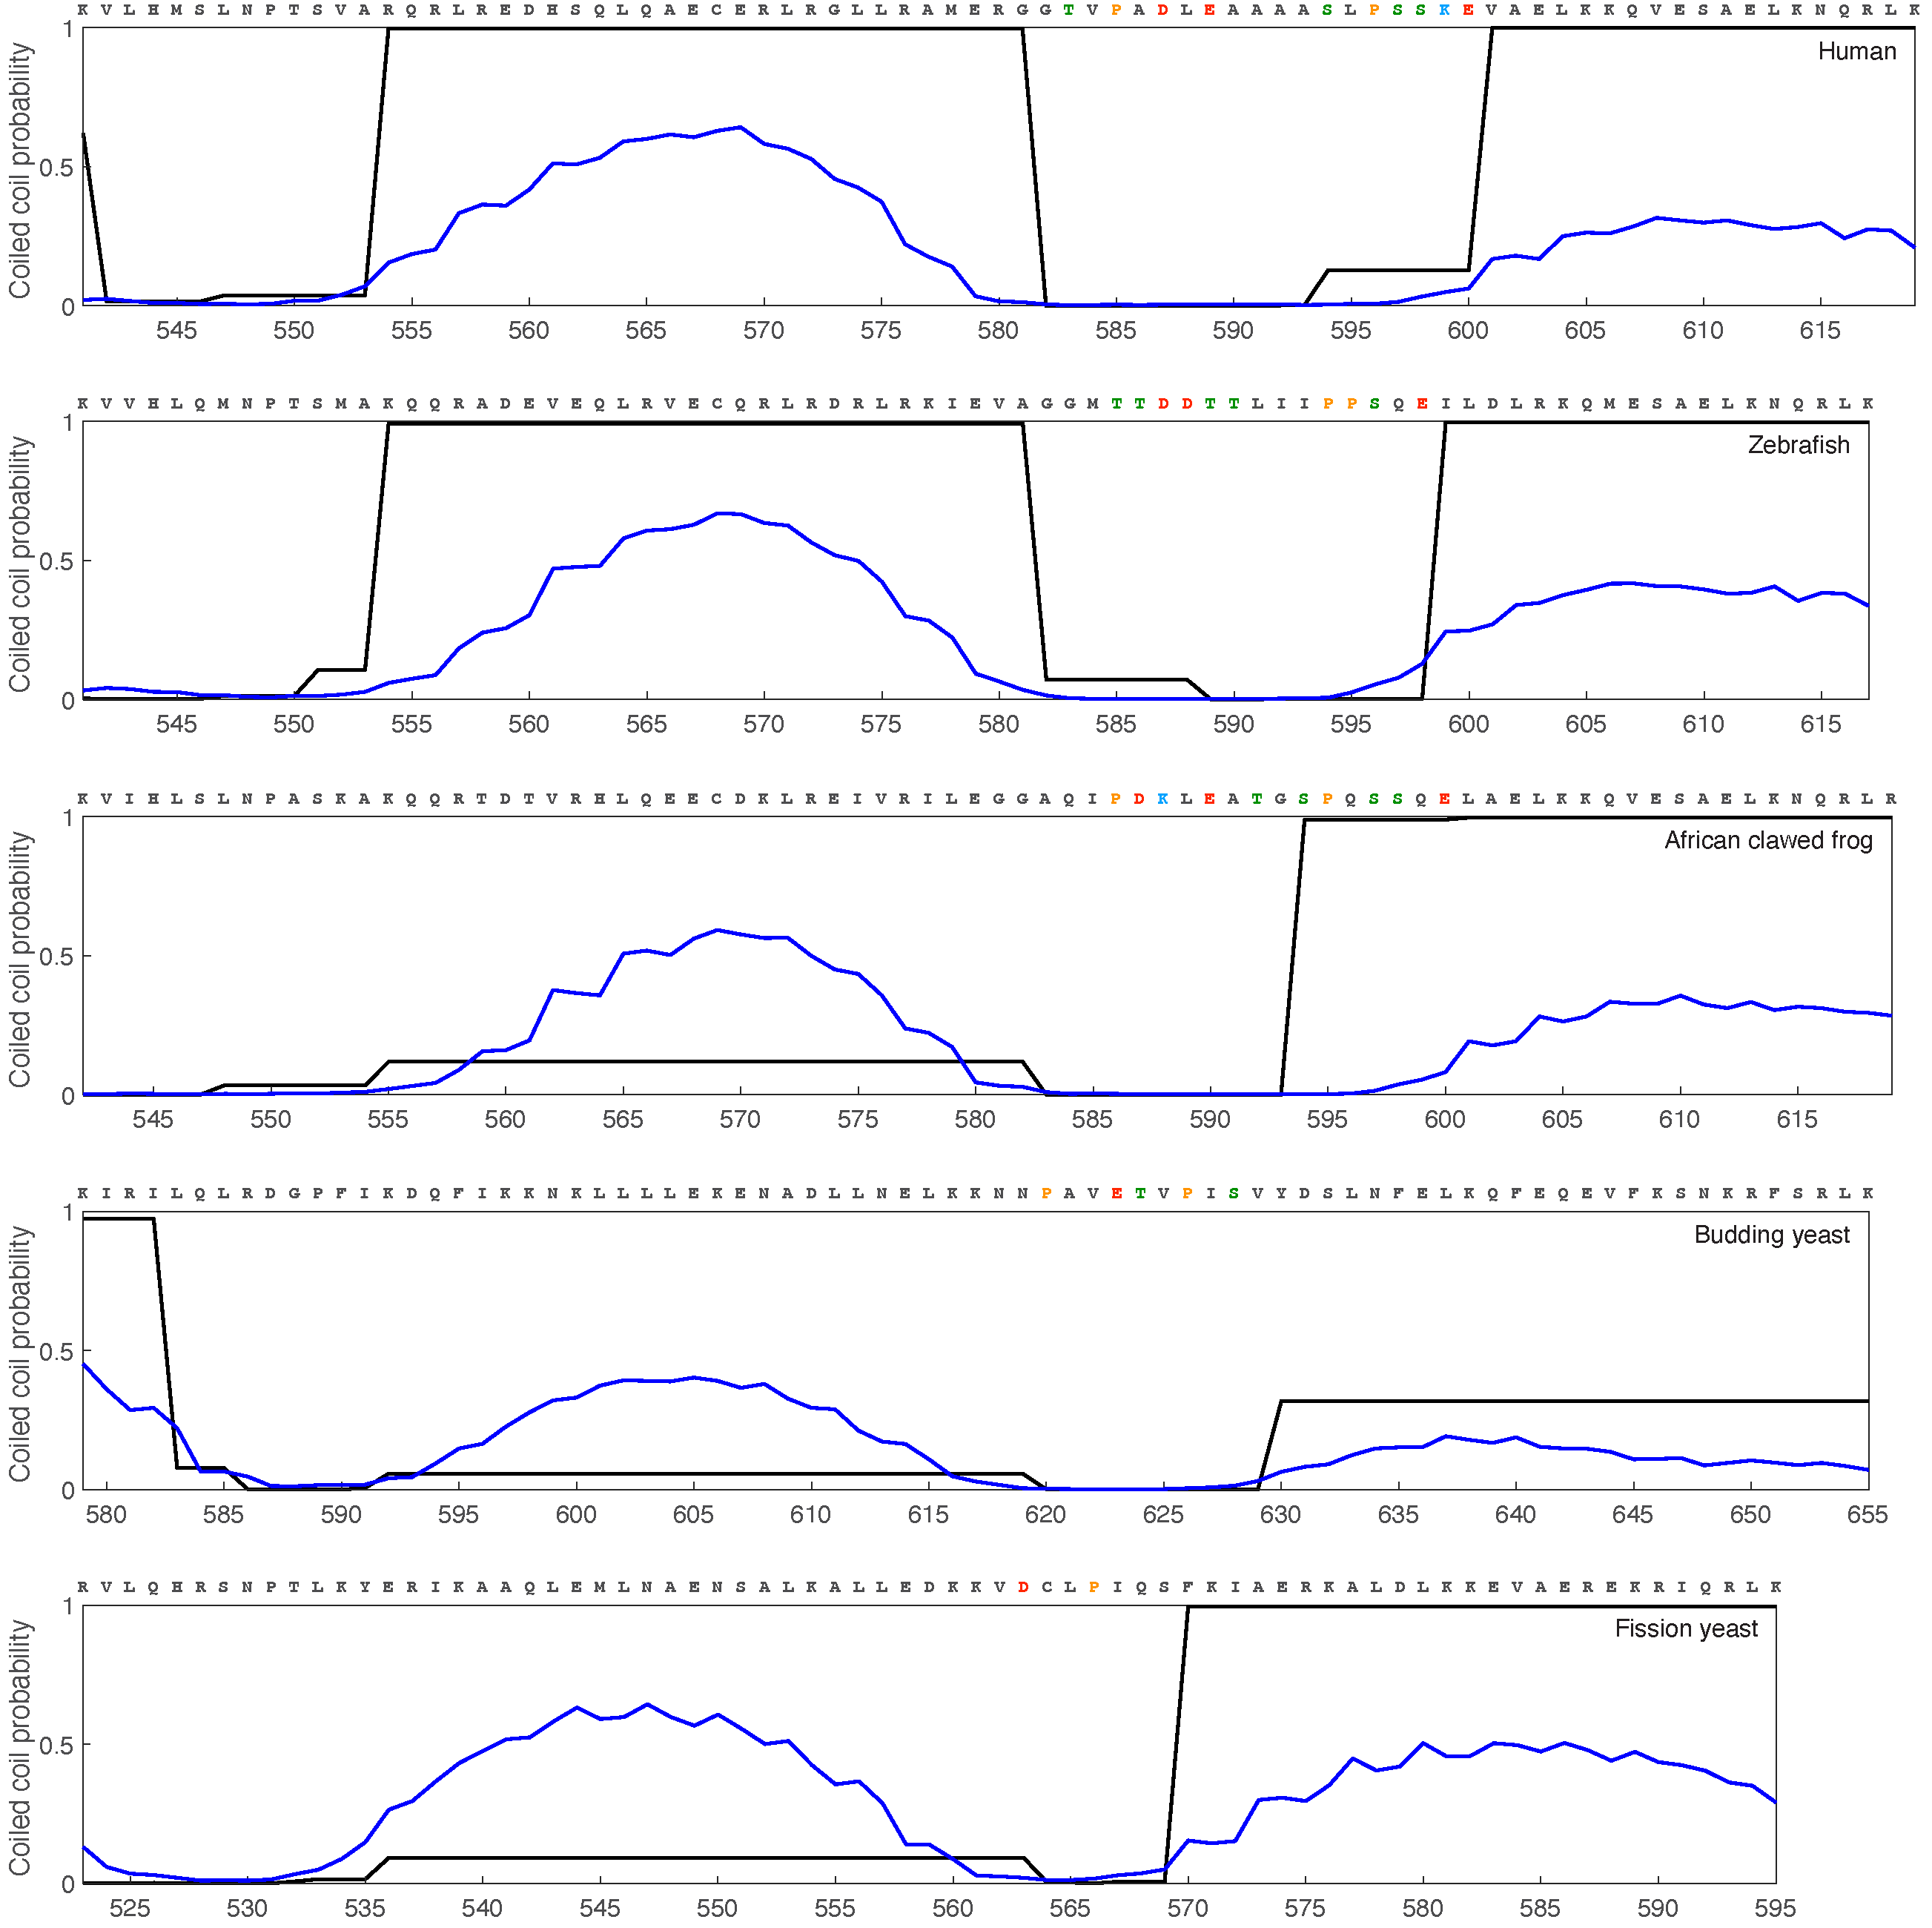
\includegraphics[width=\textwidth]{chapters/figures/MAD1_MIM-RLK_Lupas+DeepCoil2.pdf}
    \caption{\textbf{The secondary structure of \protein{Mad1}'s loop is conserved.}}
    \noindent\justifying The figure shows coiled coil predictions by two algorithms (black curves: Lupas' method using a gliding window size of 28 residues \cite{LupasCOILS}; blue curves: raw predicted probabilities by DeepCoil2 \cite{DeepCoil}) on the region spanning from \protein{Mad1}'s MIM (which is also not a coiled coil \cite{Structure1GO4}) to \protein{Mad1}'s consensus RLK motif from \Latin{Homo sapiens} (human), \Latin{Danio rerio} (zebrafish), \Latin{Xenopus Laevis} (African clawed frog), \Latin{Saccharomyces cerevisiae} (budding yeast), and \Latin{Schizosaccharomyces pombe} (fission yeast). The $x$-axis represents the coordinates of residues within \protein{Mad1}. The primary sequences of full-length \protein{Mad1} proteins were supplied as the input, but only probability predictions on this region are shown here. The RLK motif directly binds to \protein{Bub1} \cite{Ji2017eLife, MAD1CStructure} and is located within the coiled coil leading to the RWD domain (see the crystal structure on the right in \myref{HsMAD1CTerStructure}). Residues within the putative loop region are colored as in \myref{HsMAD1CTerStructure}.
    \label{MAD1_MIM-RLK_Lupas+DeepCoil2}
\end{figure}

\section{\protein{Mad1}'s loop region is important to the SAC signaling activity \Latin{in vivo}}
\label{LoopDeletionSection}

Now that we had shown that the \protein{Mad1}-\protein{Mad2} heterotetramer can assume a fold-back conformation likely enabled by the loop region of \protein{Mad1}, we next sought to determine whether the loop region is important to the SAC signaling activity \Latin{in vivo}. We integrated the expression cassette of either \protein{Mad1}-mNG or \protein{Mad1}\textDelta{}L-mNG under the regulation of a TRE into the genome of HeLa-A12 cells using Cre-\bacterialgene{lox} RMCE (see \myref{Cre-lox}). We then knocked down endogenous \protein{Mad1} in these stably-transfected cells using siRNAs that target the 3'-UTR of \gene{Mad1} \cite{siMAD1-3UTR} (henceforth collectively referred to as si\gene{Mad1}) and induced the expression of \protein{Mad1}(WT/\textDelta{}L)-mNG (si\gene{Mad1}-resistant due to their lack of the endogenous 3'-UTR) by doxycycline. Similar to \myref{per_se}, we used our genome-edited \gene{Mad1}-mNG HeLa-A12 cell line as a reference of the endogenous level of \protein{Mad1} in our live-cell fluorescence imaging.

We found out that knocking down \gene{Mad1} using si\gene{Mad1} for two days indeed crippled the SAC signaling activity. However, cells with less than 10\% of the physiological level of \protein{Mad1} (estimated from the immunoblot in \myref{MAD1Rescue_WB}) still arrested in mitosis for a significant amount of time in \SI{100}{nM} nocodazole (only about two hours less than the control group with a physiological level of \protein{Mad1}), indicating that even a small pool of \protein{Mad1} could sustain a considerable level of SAC signaling activity.

% figure
% \myref{MAD1Rescue_WB}
% add t-test between knockdown and knockdown + ∆L

Surprisingly, \protein{Mad1}\textDelta{}L had impaired support for the SAC in a dominant-negative manner. That is, cells which had most of its endogenous \protein{Mad1} knocked down and were rescued by a physiological level of \protein{Mad1}\textDelta{}L arrested in mitosis for a significantly shorter duration than cells which had most of its endogenous \protein{Mad1} knocked down but were not rescued. One possible explanation was that the recombinant \protein{Mad1}\textDelta{}L-mNG dimerized with the remaining endogenous \protein{Mad1} and restricted its structural flexibility. Indeed, as predicted by ColabFold advanced, all five models of the heterodimer between the C-terminus of wildtype \protein{Mad1} and the C-terminus of \protein{Mad1}\textDelta{}L were in a similar conformation, wherein the loop of the wildtype \protein{Mad1} introduced a kink in the overall structure of the heterodimer but not enabling fold-back. To confirm this hypothesis, we pulled down doxycycline-induced \protein{Mad1}(wildtype/\textDelta{}L)-mNG in HeLa-A12 cells wherein the endogenous \protein{Mad1} was not knocked down. And indeed, we found that endogenous \protein{Mad1} was also pulled down by both \protein{Mad1}-mNG and \protein{Mad1}\textDelta{}L-mNG, but not by mNeonGreen alone.

To confirm that the defect in the SAC signaling activity observed in cells rescued by \protein{Mad1}\textDelta{}L was not due to \protein{Mad1}\textDelta{}L's potential defective interaction with \protein{Mad2} or any unexpected change in the expression level of certain SAC proteins, we quantified the localization of \protein{Mad2} at signaling kinetochores by fluorescence imaging and quantified the expression level of other SAC proteins by immunoblot. Genome-edited \protein{Mad2}^mScarlet-I HeLa-A12 cells which had most of its endogenous \protein{Mad1} knocked down and rescued by \protein{Mad1}(wildtype/\textDelta{}L)-mNG showed that no difference in the localization of either \protein{Mad1} or \protein{Mad2} at signaling kinetochores when treated by \SI{330}{nM} nocodazole. The cellular abundance of some other SAC proteins like \protein{BubR1}, \protein{Cdc20}, and \protein{Bub3} was also not affected by the rescue experiment (see \myref{MAD1Rescue_WB}).

\Latin{In vitro} reconstitution data (not shown here) from our collaborator also suggested that truncating the loop region of \protein{Mad1} reduced the rate of the MCC's assembly, as quantified by a FRET-based assay \cite{Faesen2017, BUB1-CDC20-MAD1}. Although the results of our knockdown-rescue experiment may have been influenced by the incomplete knockdown of the endogenous \protein{Mad1}, all of these experiments together proved that the loop region of \protein{Mad1} is critical to the SAC signaling activity in its own right.